\chapter{Representação Intermediária de Código}\label{ch:IR}

Na computação, um compilador é um programa responsável por traduzir um código escrito em uma linguagem de programação para outra, geralmente do código-fonte para código de máquina, permitindo assim a execução do programa.
Durante esse processo, é fundamental que o mínimo de informações seja perdido, uma vez que a semântica original deve ser preservada no processo de tradução.
Uma abordagem comum utilizada para manter a integridade semântica e possibilitar otimizações, são as representações intermediárias (IR, do inglês \textit{intermediate representation}) \cite{cooper2014}.

Compiladores modernos, amplamente utilizados na indústria, empregam mais de uma IR para tirar proveito das vantagens de cada uma, uma vez que essas representações são projetadas para diferentes objetivos, como otimizações específicas.
As IRs podem ser classificadas de acordo com o nível de abstração e são comumente aplicados em sequência.
Representações com um nível maior de abstração são usadas próximas ao código-fonte, enquanto aquelas de nível mais baixo estão mais próximas do código de máquina \cite{aho2008compilers}, como ilustrado na figura \ref{fig:abstraction-level-irs}.

\begin{figure}
  \centering
  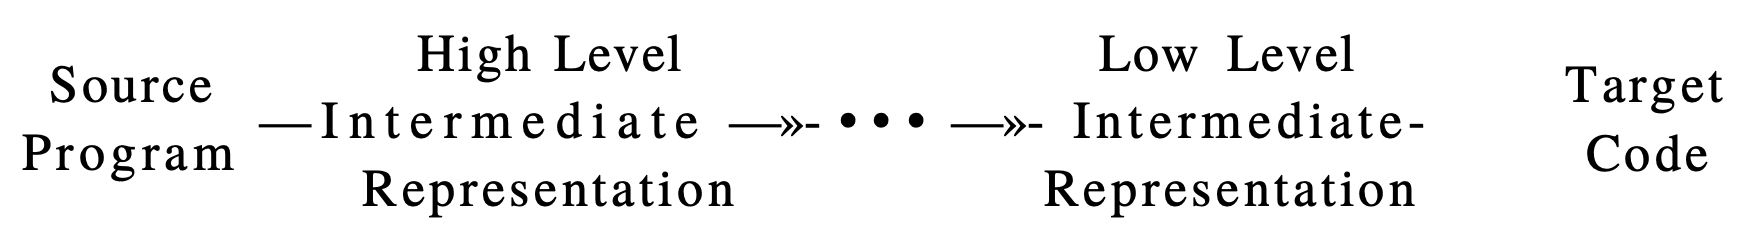
\includegraphics[width=.7\textwidth]{Imagens/abstraction-level-irs.png}
  \caption{Sequência de representações intermediárias}
  \label{fig:abstraction-level-irs}
  \small{Fonte: \cite{aho2008compilers}}
\end{figure}

Uma das principais informações que deve ser preservada em uma IR, é o fluxo de controle, isto é, a ordem em que as instruções do programa são executadas, como chamadas de função, \textit{loops} e condições.
Para garantir que o compilador mantenha a semântica correta do programa, o fluxo de controle deve ser repassado de alguma maneira durante o processo de tradução \cite{cooper2014}.
Uma das maneiras disso ser feito explicitamente, é com o uso de continuações, que são funções que descrevem o próximo passo de uma computação em um ponto particular da execução do programa.

\section{CPS}\label{sec:cps}

O estilo de passagem de continuações (CPS, do inglês \textit{continuation passing style}) é uma técnica de transformação de código que torna o fluxo de controle de um programa explícito, ao converter o estilo convencional de chamadas de função em chamadas que passam explicitamente o controle para a próxima etapa, conhecida como continuação (do inglês, \textit{continuation}) \cite{appel1992compiling}.
Em vez de retornar diretamente o resultado de uma função, o CPS transforma cada função para que, ao finalizar sua computação, ela invoque uma \textit{continuation}, que representa o próximo passo a ser executado no programa.

O cálculo lambda, definido por \citeonline{church1932set}, é um sistema formal que serve como base para a maioria das linguagens funcionais.
Ele é capaz de representar qualquer computação utilizando abstrações e aplicações através de reduções.
Sua sintaxe consiste em três regras simples que definem os elementos principais do sistema: variável, abstração e aplicação, conforme apresentados a seguir:

\begin{equation} \label{eq:lambda-calculus}
  e ::= x \mid \lambda x. e \mid e e
\end{equation}

A partir dessa sintaxe, um termo $e$ pode possuir apenas uma das três formas.
A primeira forma refere-se às variáveis, que representam identificadores no sistema.
A segunda forma, chamada de abstração, define uma função lambda: uma função que associa o identificador $x$ a um termo $e$, seu corpo, com $x$ vinculado ao termo $e$.
Finalmente, a aplicação ocorre quando um termo $e$ é aplicado a outro $e$, representando a chamada de uma função.

Para avaliar expressões no cálculo lambda, usamos três tipos de redução: $\alpha$, $\beta$ e $\eta$, que seguem as seguintes definições:

\begin{description}
  \item[$\alpha$-redução:] Renomeação de variáveis ligadas.
        \begin{align}
          \lambda x . e[x] & \rightarrow \lambda y . e[y] \label{eq:alpha-reduction}
        \end{align}

  \item[$\beta$-redução:] Aplicação de função.
        \begin{align}
          (\lambda x . e_1) e_2 & \rightarrow e_1 [e_2 / x] \label{eq:beta-reduction}
        \end{align}

  \item[$\eta$-redução:] Expansão de função.
        \begin{align}
          \lambda x . (e \, x) & \rightarrow e \quad \text{se } x \text{ não ocorre livre em } e \label{eq:eta-reduction}
        \end{align}
\end{description}

As reduções são responsáveis pela semântica operacional do cálculo lambda.
A $\alpha$-redução permite a renomeação de variáveis ligadas, enquanto a $\beta$-redução descreve a aplicação de funções, substituindo o parâmetro da função por um valor passado como argumento.
Por fim, a $\eta$-redução lida com a simplificação de funções quando elas aplicam diretamente seu argumento.

A transformação para CPS se baseia nessa estrutura formal.
No cálculo lambda tradicional, o fluxo de execução é implícito: as funções são aplicadas e seus resultados são retornados automaticamente.
No entanto, no CPS, o fluxo de controle é explicitamente representado como uma série de chamadas a funções.
Cada função, em vez de retornar diretamente um valor, recebe um argumento extra, a continuação, que indica o próximo passo da computação.

Por exemplo, a expressão $\lambda x. x + 1$ no cálculo lambda tradicional retornaria o valor $x + 1$. Ao transformar essa expressão para CPS, ela se torna $\lambda x. \lambda k. k (x + 1)$.

Aqui, $k$ é a continuação que processa o resultado $x + 1$.
Essa técnica é especialmente poderosa no contexto de compiladores, uma vez que facilita várias formas de otimizações e análises, como eliminação de chamadas de função (TCO, do inglês \textit{tail-call optimization}), expansão \textit{inline}, representação de \textit{closures}, alocação de registradores, entre outras \cite{appel1992compiling}.
Ao transformar o código para CPS, todo o fluxo de execução do programa é capturado como uma série de chamadas encadeadas de funções, sem depender de uma pilha de execução implícita.

O cálculo de continuações (do inglês, \textit{CPS-calculus}), conforme definido por \citeonline{thielecke1997}, é um sistema formal que leva o CPS além de seu uso tradicional como uma técnica de transformação de código, tratando-o como um modelo computacional por si só.
Enquanto o CPS é utilizado como uma IR em compiladores, o cálculo de continuações oferece uma estrutura para raciocinar formalmente sobre computações onde o fluxo de controle é explicitamente representado.
Os termos do cálculo de continuações, chamados de comandos, são descritos pelas seguintes regras:

% Sintaxe do cálculo de continuações (o ideal seria a que o cristiano pediu, mas enquanto não achar vai a do Thielecke msm)
\begin{equation}
  M ::= x\langle \vec{x} \rangle \mid M\{x\langle \vec{x} \rangle = M\}
\end{equation}

Aqui, $x\langle \vec{x} \rangle$ representa um salto (\textit{jump}), isto é, uma chamada para a continuação $x$ com os parâmetros $\vec{x}$, sendo essencialmente uma chamada direta para a continuação, enquanto $M\{x\langle \vec{x} \rangle = M\}$ representa um vínculo (\textit{binding}), onde o corpo $M$ está vinculado à continuação $x$ com os parâmetros $\vec{x}$, isto é, uma chamada intermediária que, ao ser chamada, executará o próximo passo da computação.
% Explicar a sintaxe e a transformação para CPS, contendo exemplos em Haskell.


% KARLA STUFF

% \subsection{Grafo de Fluxo de Controle}\label{sub:gfc}
% Uma IR baseada em controle e análise de fluxo de dados é capaz de capturar informações sobre o fluxo de dados ao longo dos caminhos de execução do programa e verificar as alterações nos fluxos de controle geradas a partir de expressões booleanas \cite{aho2008compilers}. Estas informações permitem que uma série de otimizações sejam aplicadas sobre o programa (e.g., eliminação de fluxo de controle inútil e eliminação de sub-expressão comum).

% O grafo de fluxo de controle (do inglês, \textit{control flow graph}, ou CFG) é um exemplo de IR para análise de controle e fluxo de dados modelado como um grafo dirigido $G=(N,E)$, representando, respectivamente, blocos de código básicos $n$, de forma que $n \in N$, e a transferência de controles de um bloco a outro, modelado como uma aresta $e$, tal que $e \in E$. Um bloco básico é uma sequência linear de código onde não ocorrem ramificações no grafo, podendo representar mais de uma linha do código-fonte traduzido, como mostra a figura \ref{fig:cfg-if} \cite{allen1970control}.

% \begin{figure}
%     \centering
%     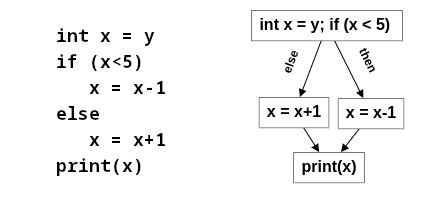
\includegraphics[width=.7\textwidth]{Imagens/cfg2.png}
%     \caption{Modelagem de \textit{If Statement} em CFG}
%     \small{Fonte: \me }
%     \label{fig:cfg-if}
% \end{figure}

% Uma das características mais comuns em CFGs são as ramificações. Elas irão ocorrer sempre que uma expressão booleana for avaliada pelo programa, como demonstrado na figura \ref{fig:cfg-while}, onde (\verb|a < 10|) é avaliado e o fluxo é ramificado para (\verb|print "saiu"|) e (\verb|print "ok"|). Além disso, a figura \ref{fig:cfg-while} também apresenta um loop no grafo, identificado por meio da revisitação do nó (\verb|while a < 10|) partindo de si, o que representa um laço de repetição no programa-fonte. Além das ramificações de saída, é possível que um nó seja alcançado por mais de um nó predecessor, como mostra a figura \ref{fig:cfg-if}, onde (\verb|print(x)|) pode ser acessado pelos nós (\verb|x = x+1|) e (\verb|x = x-1|).

% \begin{figure}
%     \centering
%     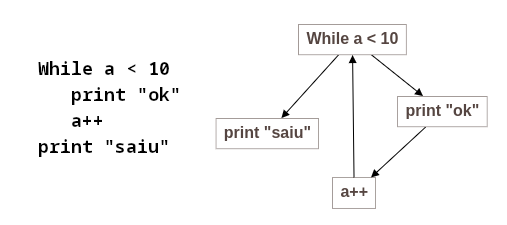
\includegraphics[width=.7\textwidth]{Imagens/cfg.png}
%     \caption{Modelagem de \textit{While Statement} em CFG}
%     \small{Fonte: \me }
%     \label{fig:cfg-while}
% \end{figure}

% Dentre as opções de modelagem possíveis para um CFG, a escolha de tipo de bloco a ser implementado é de extrema importância. É possível utilizar blocos de instrução única em substituição a implementação comum de bloco básico, como no caso apresentado na figura \ref{fig:cfg-while}, onde cada bloco representa uma única instrução independente de gerar ramificação no grafo ou não. Essa escolha de projeto pode simplificar algoritmos para análise e otimização, contudo utiliza mais memória e leva mais tempo para percorrer do que a modelagem utilizando blocos básicos.

% Um compilador pode utilizar um CFG, explicita ou implicitamente, em diversas etapas para auxiliar no processo de otimização por análise de fluxos. Outros grafos também podem ser derivados a partir do CFG, fornecendo diferentes tipos de informações que auxiliam na realização de análises mais profundas (e.g., grafo de dependência e grafo de chamada). Para além das derivações, CFGs também podem possuir casos específicos, com regras próprias, assim como os casos de atribuição estática única.


% \subsection{Forma de Atribuição Estática Única}\label{sub:ssa}

% A forma de atribuição estática única (do inglês, \textit{static single assignment}, ou SSA) representa uma particularidade de CFG bastante utilizada como IR em compiladores de linguagens imperativas. Neste formato, será permitido, somente, que cada referência a uma variável esteja relacionada a uma única atribuição. Para que essa propriedade seja mantida é necessário um procedimento de renomeação de todas as variáveis com mais de uma atribuição no código base.

% \begin{figure}
%     \centering
%     \includegraphics[width=.5\textwidth]{Imagens/SSA.png}
%     \caption{Modelagem de \textit{If Statement} em SSA}
%     \small{Fonte: \me}
%     \label{fig:ssa}
% \end{figure}

% A figura \ref{fig:ssa} apresenta a modelagem do mesmo código representado anteriormente pela figura \ref{fig:cfg-if}, porém agora em sua forma SSA. É possível notar que a variável \verb|x|, utilizada diversas vezes no trecho de código base, foi subdividida em outras quatro variáveis (\verb|x_0|, \verb|x_1|, \verb|x_2|, \verb|x_3|) fragmentadas de modo a estabelecer o critério de atribuição única. Ao renomear estas variáveis, surge o problema de mais de um fluxo convergindo para um mesmo bloco, assim como em (\verb|print(x)|) apresentado na figura \ref{fig:cfg-if}. Este bloco de código é diretamente dependente de seus dois blocos predecessores. Na forma SSA, para decidir qual variável deve ser utilizada, dentre \verb|x_1| e \verb|x_2|, uma função $\phi$ é implementada.

% Uma função $\phi$ recebe como entrada as atribuições provenientes de diferentes arestas que fluem para um mesmo bloco. Quando o fluxo de controle passa para este bloco, a função é executada e o retorno será obtido a partir da aresta pela qual o controle entrou no bloco. Durante a passagem do código base para a forma SSA, o algoritmo deve ser capaz de renomear todas as variáveis alteradas e inserir funções $\phi$ em cada ponto de junção do CFG de forma eficiente. Para gerar uma representação SSA eficiente é necessário que as funções $\phi$ sejam colocadas somente onde é necessário, pois o excesso destas funções aumenta o custo de qualquer algoritmo que precise percorrer grafo na forma SSA.


% \begin{figure}
%     \centering
%     \includegraphics[width=.3\textwidth]{Imagens/blocos.png}
%     \caption{Renomeação de blocos da Figura \ref{fig:cfg-if}}
%     \small{Fonte: \me}
%     \label{fig:blocos}
% \end{figure}

% Uma maneira de auxiliar o algoritmo para criar a forma SSA com um número menor de funções é realizar uma análise de dominância entre os blocos. A partir da Figura \ref{fig:cfg-if}, renomeando os blocos e abstraindo-se das informações internas a ele, foram criadas a tabela de dominância (Tabela \ref{tab:dom}) e a árvore de dominadores (Figura \ref{fig:arvore}) para o CFG. A tabela \ref{tab:dom} nos apresenta dois conceitos: dominância, dado por $D_{OM}(n)$, onde $m\in D_{OM}(n)$ se, para alcançar $n$ é \textit{necessário} passar por $m$; e dominante imediato, dado por $ID_{OM}(n)$, de forma que se $m\in D_{OM}(n)$ e $m$ é o nó mais próximo de $n$ neste conjunto, com $m \neq n$, então $m$ é o dominante imediato de $n$. Se $m \in D_{OM}(n)$ e $m\neq n$ então $m$ domina estritamente $n$, denotado por $m\gg n$.


% %tabela de dominadores
% \begin{table}
%     \centering
%     \begin{tabular}{ccccc}
%                   & A     & B       & C       & D       \\
%         $D_{OM}$  & \{A\} & \{A,B\} & \{A,C\} & \{A,D\} \\
%         $ID_{OM}$ & --    & A       & A       & A       \\
%     \end{tabular}
%     \caption{Tabela de dominância}
%     \small{Fonte: \me}
%     \label{tab:dom}
% \end{table}

% Partindo da tabela de dominância é possível criar a árvore de dominadores, de forma que se $m\in ID_{OM}$ então existe uma aresta direcionada saindo de $m$ para $n$. Como o bloco de entrada do grafo de fluxo não possui dominante imediato, este bloco será a raiz da árvore de dominadores.

% \begin{figure}
%     \centering
%     \includegraphics[width=.4\textwidth]{Imagens/arvore-dominancia.png}
%     \caption{Árvore de dominadores}
%     \label{fig:arvore}
% \end{figure}

% %esse paragrafo tem que rever

% O próximo passo é calcular as fronteiras de dominância, ou DF, para cada nó no grafo como apresentada pela tabela \ref{tab:df}. A fronteira de dominância de um dado nó $n$ é dada por todo nó $m$ no grafo, de modo que $n$ domina um predecessor de $m$, mas não domina estritamente $m$ \cite{cytron1989efficient}.

% %Tenho que ver essa fromula aqui tbm... 

% \begin{equation}
%     \begin{matrix}
%         DF(n) = \{m & | & (\exists P \in Pred(m)) & (n \in D_{om}(P) & e & n \not\gg m)\}
%     \end{matrix}
% \end{equation}

% %tabela de fronteira de dominancia
% % nao sei ainda como fica
% \begin{table}
%     \centering
%     \begin{tabular}{ccccc}
%              & A  & B     & C     & D  \\
%         $DF$ & -- & \{D\} & \{D\} & -- \\
%     \end{tabular}
%     \caption{Tabela de fronteira de dominância}
%     \small{Fonte: \me}
%     \label{tab:df}
% \end{table}

% Obtidas as fronteiras de dominância, o posicionamento de funções $\phi$ no grafo torna-se trivial. Se existe uma definição de \verb|x| no nó $n$, então deverá existir uma função $\phi$ em cada bloco pertencente a $DF(n)$. O procedimento de cálculo de fronteiras de dominância é uma forma básica de melhorar a representação na forma SSA, podendo ser utilizado por outros algoritmos para tornar a inserção de funções $\phi$ ainda mais eficiente.

% \subsection{Forma-Normal-A}\label{sub:anf}

% A utilização de IRs baseadas em $\lambda$-cálculo ocorre em diversos compiladores para linguagens funcionais. No trabalho de \citeonline{appel1987standard}, um tipo de $\lambda$-cálculo modificado é utilizado como IR em um compilador padrão para a linguagem funcional ML. Definido por \citeonline{church1932set}, o $\lambda$-cálculo puro é a representação de aplicações de funções, variáveis e abstrações.

% \begin{flushleft}
%     \qquad\qquad M := (M M) \hspace{20ex} (Aplicação)\\
%     \qquad\qquad\qquad | ($\lambda$x.M) \hspace{19ex} (Abstração)\\
%     \qquad\qquad\qquad | x  \hspace{25ex} (Variável)\\
% \end{flushleft}


% Um termo em $\lambda$-cálculo pode ser, portanto, a aplicação de um termo sobre outro, uma abstração ou uma variável. Em uma abstração do tipo ($\lambda x.M$), é dito que a variável $x$ está ligada ao termo $M$ e toda ocorrência de uma variável dentro de $M$ que não está ligada é uma variável livre. O conjunto de variáveis livres de um termo $M$ é definido como $FV(M)$.

% Em um termo em $\lambda$-cálculo é possível aplicar substituições. Uma substituição é representada como $M[x:=N]$, de forma que toda ocorrência de $x$ em $M$ será substituída por $N$. Outro conceito, para além da substituição, é a noção de termos $\alpha$-equivalentes. É possível demonstrar a equivalência entre dois termos a partir da mudança de variáveis que estão ligadas em uma abstração, e.g., os termos ($\lambda x.x$) e ($\lambda y.y$) são $\alpha$-equivalentes, pois, apenas trocando o nome de suas variáveis ligadas, podemos chegar de um termo a outro. Esta mudança de variáveis ligadas é chamada de $\alpha$-conversão ou $\alpha$-redução. Uma aplicação bastante comum de substituição e $\alpha$-conversão é o uso em $\beta$-reduções. Uma $\beta$-redução ocorre sempre que uma abstração recebe argumentos, ou seja, a função é aplicada a seus argumentos.

% \begin{center}
%     ($\lambda$x.M) N := M[x:=N] \qquad \qquad ($\beta$-redução)
% \end{center}

% Caso uma variável que ocorre livre em N apareça em alguma $\lambda$-abstração de M, então uma $\alpha$-conversão deve ser feita no termo antes de aplicar a substituição, para que assim não ocorra a ligação desta variável. Por exemplo, a $\beta$-redução do termo (($\lambda x\lambda y. x$)$y$) será ($\lambda z. y$), com a mudança da variável ligada de $y$ para $z$.

% Outra redução bastante utilizada em $\lambda$-termos é a $\eta$-redução, que ocorre como uma noção de extensionalidade. Nesta redução uma abstração do tipo ($\lambda x. f x$) é convertida apenas para $f$, desde que $x \not\in FV(f)$. Isso ocorre pela consideração de equivalência entre termos que ao serem aplicados geram o mesmo resultado. Adicionalmente, existe a possibilidade de incrementar o $\lambda$-cálculo com a definição de contextos. Um contexto é um termo com um "buraco", representado por "[]", que pode ser preenchido por uma sub-expressão. O ato de fazer este preenchimento é chamado de \textit{filling}, e.g., o \textit{filling} do contexto ($\lambda x. y []$) com o termo ($\lambda z.x$) é o termo ($\lambda x. y (\lambda z.x)$). O preenchimento acontece entre um contexto e um termo e resulta também em um termo, podendo ligar variáveis que antes eram livres. A classe sintática que define a gramática para contextos é apresentada a seguir.

% \begin{center}
%     E = [] | E ([] M)
% \end{center}

% A forma-normal-A (do inglês, \textit{Administrative normal form}, ou ANF) é uma versão de cálculo lambda utilizada como IR. Um $\lambda$-termo estará em ANF se não puderem ser aplicadas mais reduções do tipo A. \citeonline{sabyr1992} definem o conjunto de reduções A pelas regras:

% \begin{flushleft}
%     \qquad\qquad $E[((\lambda x.M) N)] \longrightarrow ((\lambda x.E[M]) N)  \hspace{7ex} x \not\in FV(E) \hspace{10ex} (\beta_{lift})$

%     \qquad\qquad $E[((M N) L)] \longrightarrow ((\lambda x.E[L]) (M N))  \hspace{6ex} x \not\in FV(E,L) \hspace{8ex} (\beta_{flat})$

%     \qquad\qquad $((\lambda x.x) M) \longrightarrow M \hspace{41ex} (\beta_{id})$

%     \qquad\qquad $((\lambda x.E[(y x)]) M) \longrightarrow E[(y M)] \hspace{10ex} x \not\in FV(E[y]) \hspace{8ex} (\beta_{\Omega})$
% \end{flushleft}

% Tais regras derivam na seguinte gramática para $\lambda$-cálculo que respeita as restrições impostas por ANF:
% \\
% \\

% \verb|E := V|

% \qquad|\verb| let x = V in E|

% \qquad|\verb| let x = V V in E|

% \verb|V := x|

% \qquad| $\lambda$\verb|x. E|\\

% Além disso, \citeonline{flanagan1993essence} demonstram a equivalência entre as máquinas abstratas para compiladores que utilizam \textit{continuation-passing-style} (CPS) e ANF, sendo que a máquina abstrata para ANF utiliza um número menor de passos para alcançar o objetivo. A utilização de continuações para compilar de forma eficiente uma linguagem funcional foi apresentada, inicialmente, por \citeonline{steele1978rabbit} ao criar um compilador para Scheme (dialeto de Lisp). Entretanto, a ideia se popularizou com Appel, em seu livro "Compiling with Continuantions" \cite{appel1992compiling}. Alguns artigos na área de continuações apresentam noções de isomorfismo entre as representações já discutidas no presente trabalho. No artigo de \citeonline{kelsey1995correspondence} uma proposta de conversão de CPS para SSA é apresentada a partir de funções de tradução CPS$\longrightarrow$SSA e SSA$\longrightarrow$CPS; \citeonline{chakravarty2004functional} criam uma formalização do mapeamento de programas na forma SSA para ANF; e \citeonline{sabyr1992} comprovam a correspondência entre ANF e o $\lambda$-cálculo de Moggi, $\lambda_{c}$ \cite{moggi1988computational}.



% \section{Conversão de SSA para Código Funcional}\label{sec:conversaoSSA}
% Como visto na seção \ref{sub:ssa}, um programa em SSA terá cada variável ligada a uma única atribuição. Para que isso ocorra, é preciso renomear as variáveis utilizadas no código e implementar funções $\phi$ para definir o valor de variáveis que pertencem a pontos de junção no grafo.
% Para demonstrar a correspondência entre SSA e código funcional, \citeonline{appel1998ssa} se utiliza de alguns exemplos de códigos em SSA, o qual também será aqui utilizado. Seja o seguinte trecho de código em uma linguagem de programação qualquer:

% \begin{verbatim}
%         i <- 1
%         j <- 1
%         k <- 0
%         while k < 100
%             if j < 20
%                 j <- i
%                 k <- k + 1
%             else
%                 j <- k
%                 k <- k + 2
%         return j
%     \end{verbatim}

% \begin{figure}
%     \centering
%     \includegraphics[width=.4\textwidth]{Imagens/cfg1.png}
%     \caption{Modelagem CFG}
%     \small{Fonte: \cite{appel1998ssa}}
%     \label{fig:cfg-teste}
% \end{figure}

% \begin{figure}
%     \centering
%     \includegraphics[width=.4\textwidth]{Imagens/ssa1.png}
%     \caption{Modelagem SSA}
%     \small{Fonte: \cite{appel1998ssa}}
%     \label{fig:ssa-teste}
% \end{figure}

% Sua versão em CFG é apresentada pela figura \ref{fig:cfg-teste} e a versão em SSA pela figura \ref{fig:ssa-teste}. Outra forma de visualizar o programa na forma SSA é como um conjunto de funções mutuamente recursivas, onde cada função recebe três argumentos, com exceção da função inicial. O seguinte trecho de código funcional é uma representação correspondente a forma SSA.

% \begin{verbatim}
%         f1 = let i1 = 1
%                  j1 = 1
%                  k1 = 0
%               in f2 i2 j1 k1 
%         f2 i2 j2 k2 = if k2 < 100 then (f3 i3 j3 k3) else (f4 i2 j2 k2)
%         f3 i3 j3 k3 = if j3 < 20 then (f5 i3 j3 k3) else (f6 i3 j3 k3)
%         f4 i4 j4 k4 = j4
%         f5 i5 j5 k5 = let j8 = i5
%                           k8 = k5 + 1
%                       in (f7 i5 j8 k8)
%         f6 i6 j6 k6 = let j9 = k6
%                           k9 = k6 + 2
%                       in (f7 i6 j9 k9)
%         f7 i7 j7 k7 = (f2 i7 j7 k7)
%     \end{verbatim}

% Entretanto, o repasse de argumentos nem sempre é necessário visto que muitas funções se quer utilizam estes argumentos e apenas os repassam para o próximo bloco de código. Para não haver um excesso de argumentos desnecessários é possível utilizar o conceito de funções aninhadas. Seguindo o mesmo caminho, a figura \ref{fig:ssa-teste} também possui um excesso de funções $\phi$. Colocando tais funções apenas onde necessário, chegamos a figura \ref{fig:ssa-2}, que corresponde perfeitamente ao código utilizando funções aninhadas a seguir.

% \begin{verbatim}
%         f = let i1 = 1
%                 j1 = 1
%                 k1 = 0
%             in let f2 (j2, k2) = if k2 < 100
%                                  then let f7 (j4, k4) = f2 (j4, k4)
%                                       in if j2 < 20
%                                          then let j3 = i1
%                                                   k3 = k2 + 1
%                                               in f7 (j3, k3)
%                                          else let j5 = k2
%                                                   k5 = k2 + 1
%                                               in f2 (j5, k5)
%                                  else return j2
%                in f2 (j1, k1) 
%     \end{verbatim}

% \begin{figure}
%     \centering
%     \includegraphics[width=.4\textwidth]{Imagens/ssa2.png}
%     \caption{Modelagem de SSA com o mínimo de funções $\phi$}
%     \small{Fonte: \cite{appel1998ssa}}
%     \label{fig:ssa-2}
% \end{figure}

% Dessa forma, é possível notar uma relação direta entre as funções $\phi$ e as chamadas de função no código. Apenas os blocos que utilizam funções $\phi$ possuem uma chamada de função correspondente no trecho de código.


% \section{Efeitos}\label{sec:efeitos}

% \citeonline{mitchell_2002} define um efeito colateral (do inglês, \textit{side effect}) como mudanças visíveis no estado da máquina como resultado da valoração de uma expressão. Dessa forma, duas ocorrências de uma mesma expressão podem ter resultados diferentes, não permitindo transparência referencial. Nesse contexto, ao retornar um valor não observável, consequentemente, um beta-redex $(\lambda x.a) b$ é observacionalmente distinto de um beta-reduto $a[x:=b]$ para algum efeito em $b$. A grande necessidade de IRs parte do suposto de que o $\lambda$-cálculo não trabalha bem com efeitos colaterais, podendo duplicar estes efeitos. Partindo deste pressuposto, \citeonline{moggi1988computational} propõe o $\lambda_{c}$ isomórfico a ANF e capaz de lidar bem com efeitos.]

% No campo de linguagens funcionais, existe uma divisão entre linguagens puras ou impuras. Linguagens puras utilizam $\lambda$-cálculo puro, enquanto as impuras estendem o $\lambda$-cálculo com uma série de possíveis efeitos. Porém, mesmo linguagens ditas "puras", podem, atualmente, simular e tratar estes efeitos por meio do uso de mônadas. Atualmente é possível, também, separar código puro de código com efeito colateral a partir do uso de um sistema de tipos e efeitos.

% \subsection{Mônadas}\label{sub:monadas}
% A utilização de mônadas para linguagens funcionais foi apresentada por \citeonline{wadler1995monads}, o qual incorporou o conceito proveniente do estudo de teoria das categorias. Proposta como uma forma de simular efeitos colaterais em linguagens puras, a mônada de Wadler fundamentava-se na tríade (\textit{M}, \textit{unit}, $*$). Nesta tríade, \textit{M} era o construtor de tipo da classe, \textit{unit} o encapsulamento de um dado comum em uma mônada e $*$ o mapeamento de uma função em uma mônada. As assinaturas de tipo para os dois últimos conceitos é apresentada a seguir.

% \begin{center}
%     \textit{unit :: a }$\rightarrow$\textit{ M a}\\
%     \textit{<*> :: M a }$\rightarrow$\textit{ (a }$\rightarrow$\textit{ M b) }$\rightarrow$\textit{ Mb}
% \end{center}

% Utilizando mônadas é possível simular diversos efeitos como exceções, entrada e saída, não-determinismo, entre outros. Além disso, para ser válida, é necessário que as operações de uma mônada criada siga três regras: \textit{left unit, right unit} e Associatividade.

% \begin{itemize}
%     \item \textit{Left unit:} Computar o valor de \textit{a}, ligá-lo a \textit{b} e depois computar \textit{n} é equivalente a \textit{n} com todas as ocorrências de \textit{b} substituídas por \textit{a}.
%           \begin{center}
%               \textit{unit a }$* \lambda$\textit{b. n = n[a/b] }
%           \end{center}

%     \item \textit{Right unit:} Computar \textit{m}, ligá-lo a \textit{a} e depois retornar \textit{a} é equivalente a \textit{m}.
%           \begin{center}
%               \textit{m }$* \lambda$\textit{a. unit a = m }
%           \end{center}

%     \item \textit{Associatividade:} a ordem dos parenteses neste tipo de computação é irrelevante.
%           \begin{center}
%               \textit{m }$*$ ( $\lambda$\textit{a. n }$* \lambda$\textit{b. o}) = (\textit{m }$*\lambda$\textit{a. n) }$* \lambda$\textit{b. o}
%           \end{center}
% \end{itemize}

% Wadler também apresenta formas de utilizar mônadas para trabalhar com \textit{Arrays} e implementar \textit{Parsers}.


% \subsection{Sistema de Tipos e Efeitos}\label{sub:sistemaEF}
% Outra maneira de lidar com efeitos, introduzida por \citeonline{leijen2014koka}, é o sistema de tipos e efeitos. Um sistema de tipos descreve um conjunto de regras de inferência para as construções de uma linguagem. Tais construções são formalizadas por meio de sentenças, e.g., $\Gamma \vdash M : A$, de forma que o programa $M$ possui tipo $A$ no contexto $\Gamma$ \cite{cardelli1996type}. A forma geral de uma sentença é:

% \begin{prooftree}
%     \AxiomC{$\Gamma_{1} \vdash e_{1}:\sigma_{1}$}
%     \AxiomC{...}
%     \AxiomC{$\Gamma_{n} \vdash e_{n}:\sigma_{n}$}
%     \TrinaryInfC{$\Gamma \vdash e:\sigma$}
% \end{prooftree}

% \begin{flushleft}
%     onde a parte superior da sentença é a premissa e a parte inferior é a conclusão. Tomando a formalização de sistemas de tipo como base, \citeonline{leijen2014koka} estende o modelo para apresentar efeitos. Uma sentença, neste modelo, possui a forma $\Gamma \vdash e:\sigma | \epsilon$, significando que no contexto $\Gamma$, $e$ possui tipo $\sigma$ com efeito $\epsilon$. Uma sentença geral, pode ser determinada da seguinte forma:
% \end{flushleft}


% \begin{prooftree}
%     \AxiomC{$\Gamma_{1} \vdash e_{1}:\sigma_{1} | \epsilon_{1}$}
%     \AxiomC{...}
%     \AxiomC{$\Gamma_{n} \vdash e_{n}:\sigma_{n} | \epsilon_{n}$}
%     \TrinaryInfC{$\Gamma \vdash e:\sigma | \epsilon $}
% \end{prooftree}

% O sistema de efeitos de Leijen utiliza, também, o conceito de efeitos polimórficos. Em alguns casos, o efeito de uma função é determinado a partir dos efeitos de algum de seus argumentos. Um exemplo disso é a função \textit{map}, que realiza o mapeamento de uma função sobre cada elemento de uma lista. O tipo de \textit{map} é definido como:\\

% $map : \forall \alpha \beta \mu . (list \langle \alpha \rangle, \alpha \rightarrow \mu \beta) \rightarrow \mu list \langle \beta \rangle$\\

% \begin{flushleft}
%     onde \textit{map} recebe uma lista de elementos com tipo $\alpha$ e uma função que recebe um argumento de tipo $\alpha$ e retorna um tipo $\beta$ com efeito $\mu$. Assim, \textit{map} absorve o efeito da função passada como argumento e retorna uma lista de tipo $\beta$ com efeito $\mu$. Outra característica proposta no trabalho de Leijen é o \textit{row-polymorphism} utilizando duplicação de rótulos, dessa forma $\langle exn, exn \rangle \neq \langle exn\rangle$ e a combinação de dois efeitos básicos \textit{exn} e \textit{div} gera um \textit{effect-row} $\langle exn, div \rangle$.
% \end{flushleft}

% O sistema apresentado foi implementado na linguagem de programação Koka, onde os efeitos básicos são: \textit{total, exn, div, ndet, alloc$\langle h \rangle$, read$\langle h \rangle$, write$\langle h \rangle$, io}. Sendo \textit{total} a não ocorrência de efeitos colaterais, \textit{exn} a possibilidade de exceção, \textit{div} a possibilidade de entrar em loop, \textit{ndet} para não-determinismo, \textit{alloc$\langle h \rangle$, read$\langle h \rangle$ e write$\langle h \rangle$} para representar efeitos de heap e \textit{io} para efeitos de \textit{input} e \textit{output}. Koka também utiliza, internamente, um tradutor direto de tipo que traduz um programa com efeitos para um programa monádico equivalente.

% \section{Conversão de Sistema de Efeitos para Mônadas}\label{sec:conversaoSE}
% A correspondência entre sistema de efeitos e mônadas foi observada por \citeonline{wadler2003marriage}, através da proposta de uma tradução do sistema de efeitos de \cite{talpin1992polymorphic} para mônadas. Apesar da tradução para um sistema de efeitos específico, fica implícito no trabalho que qualquer sistema de efeitos pode ser adaptado para mônadas. Seguindo esta ideia, \citeonline{vazou2016monads} formalizam a tradução do sistema de efeitos de Leijen para mônadas e vice-versa. Como grande diferencial, é apresentada a tradução de efeitos definidos pelo usuário para mônadas, assim como a tradução de \textit{row-effects} (ver sec. \ref{sub:sistemaEF}) para mônadas.

% A figura \ref{fig:conv} apresenta a conversão de uma função com o efeito \textit{amb} para código monádico equivalente. Para fazer essa passagem, o tradutor insere um \textit{bind} e passa a continuação no ponto sempre que um valor monádico é retornado. Quando um valor puro é retornado em um contexto monádico, a função \textit{unit} é utilizada, um \textit{lifting} para transformar o valor puro em uma mônada. Além disso, toda a tradução realizada baseia-se na inferência de tipos feita pelo compilador anteriormente. Dessa forma é possível determinar onde posicionar o \textit{bind} e o \textit{unit} e verificar se eles seguem ou não as leis monádicas de identidade e associatividade.

% \begin{figure}
%     \centering
%     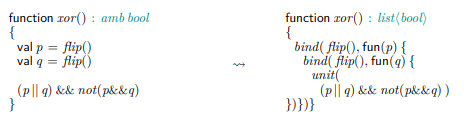
\includegraphics[width=.7\textwidth]{Imagens/conv.png}
%     \caption{Conversão de código com efeito para código monádico}
%     \small{Fonte: \cite{vazou2016monads}}
%     \label{fig:conv}
% \end{figure}

% Para lidar com polimorfismo, cada função que utiliza efeitos polimórficos recebe um dicionário como argumento extra. O dicionário vai encontrar e retornar as funções de \textit{unit} e \textit{bind} correspondentes ao efeito gerado. Quando existe a necessidade de traduzir uma função com mais de um efeito (\textit{row-effects}), uma terceira mônada é criada representando a junção destes efeitos e morfismos de \textit{lifting} de cada mônada de efeito para a mônada de junção também são criados.

